\begin{figure}[h!]
     \centering
    \captionsetup[sub]{font=small}
     \begin{minipage}[h!]{0.9\textwidth}
         \begin{subfigure}[b!]{0.3 \textwidth}
             \caption{}
             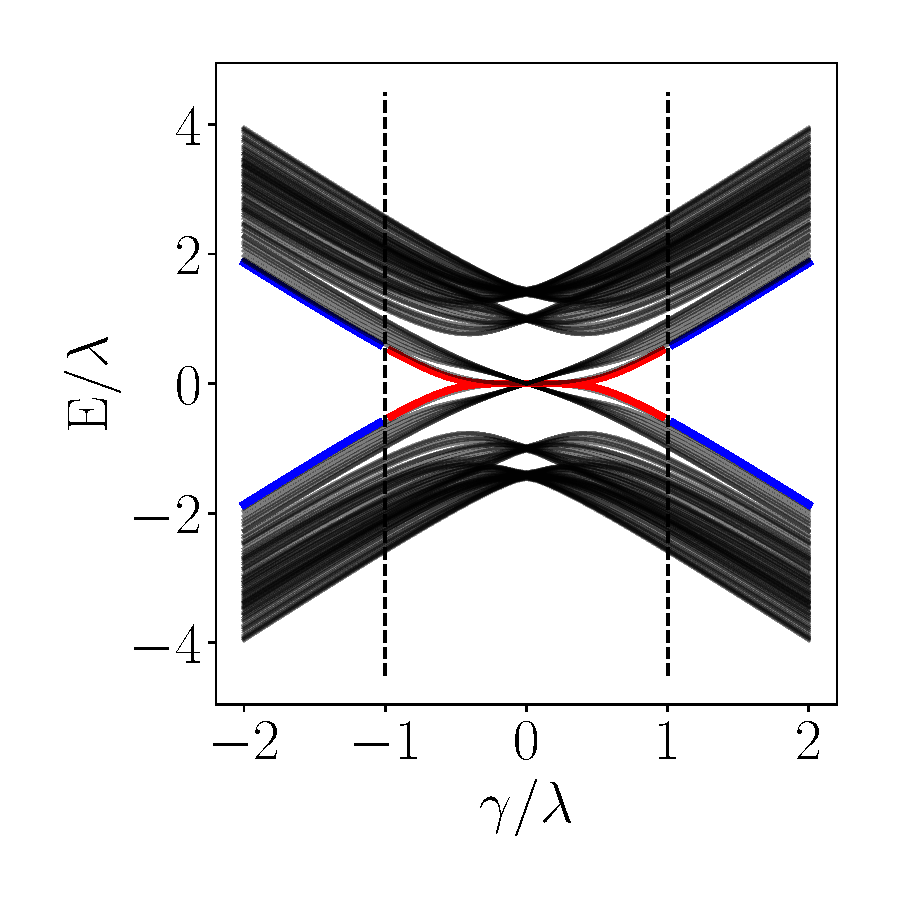
\includegraphics[width=\textwidth]{Imagenes/Resultados_Hoti_Fractal/bands_square_shh_0.05.pdf}
             \label{}
         \end{subfigure}\hspace*{-0.5em}
         \begin{subfigure}[b!]{0.3 \textwidth}
             \caption{}
             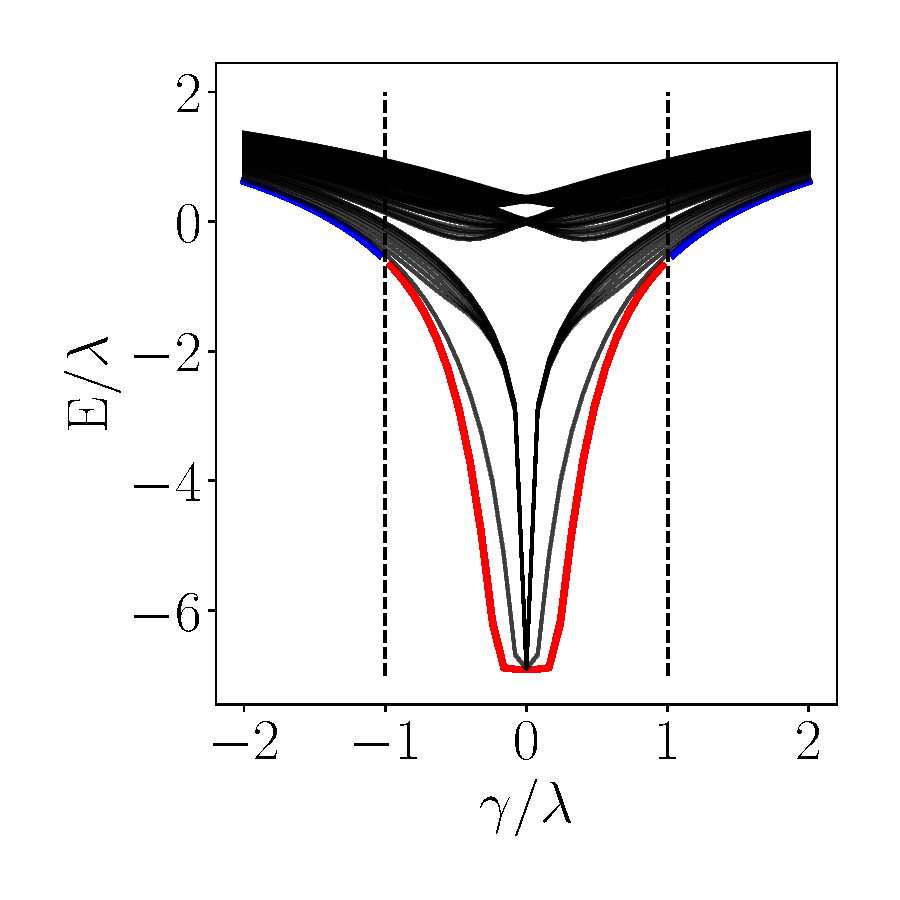
\includegraphics[width=\textwidth]{Imagenes/Resultados_Hoti_Fractal/bands_square_shh_log0.05.pdf}
             \label{}
         \end{subfigure}\hspace*{-0.5em}
         \begin{subfigure}[b!]{0.4 \textwidth}
             \caption{}
             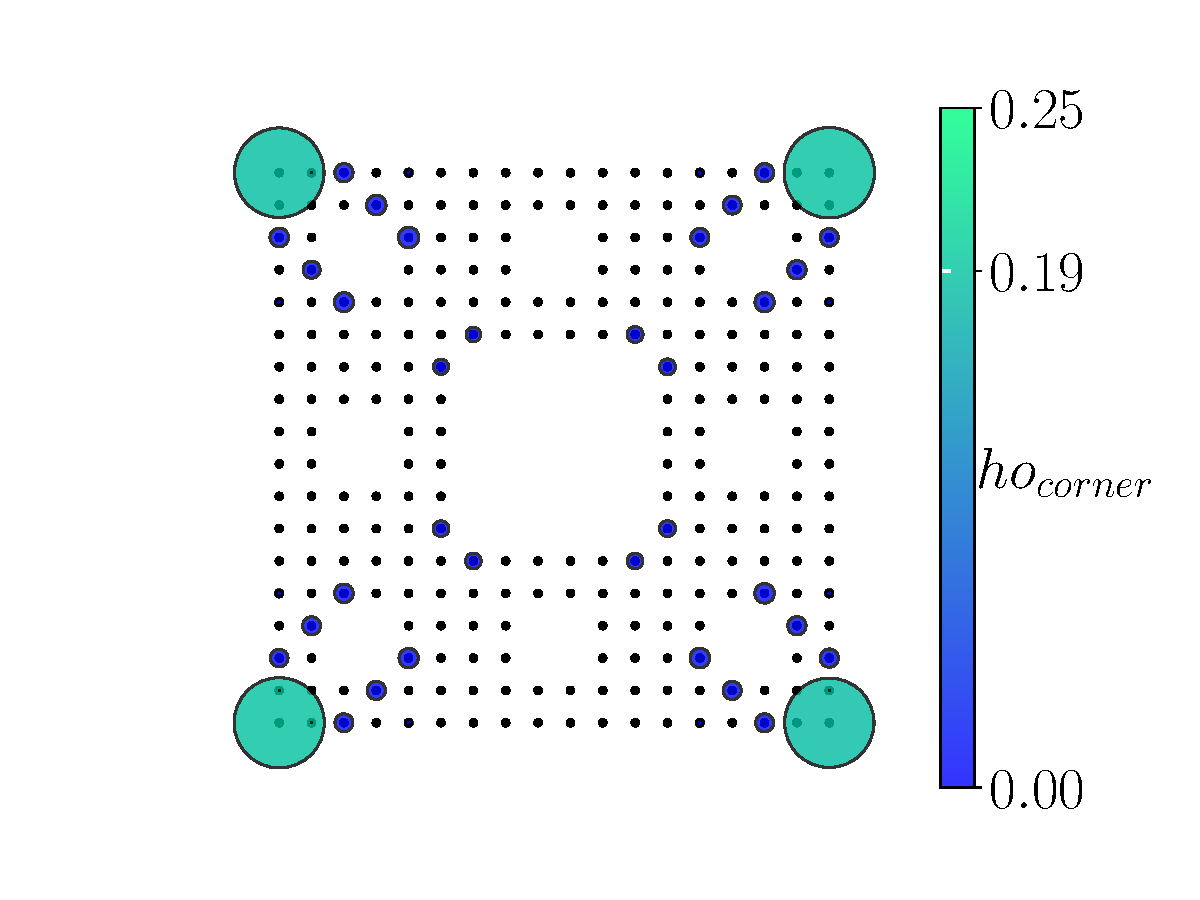
\includegraphics[width=\textwidth]{Imagenes/Resultados_Hoti_Fractal/proyection_square_0.05.pdf}
             \label{}
         \end{subfigure}\hspace*{-0.5em}
     \end{minipage}\vspace*{-2.5em}
     
     \begin{minipage}[h!]{0.9\textwidth}
         \begin{subfigure}[b!]{0.3 \textwidth}
             \caption{}
             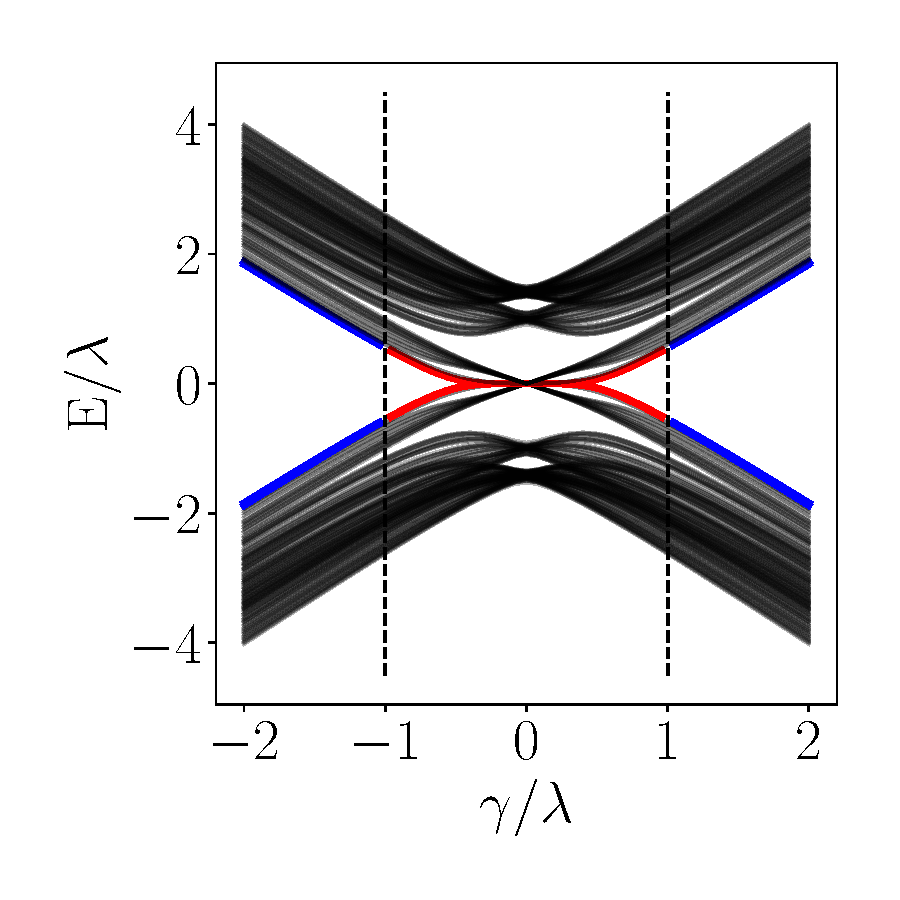
\includegraphics[width=\textwidth]{Imagenes/Resultados_Hoti_Fractal/bands_square_shh_0.1.pdf}
             \label{}
         \end{subfigure}\hspace*{-0.5em}
         \begin{subfigure}[b!]{0.3 \textwidth}
             \caption{}
             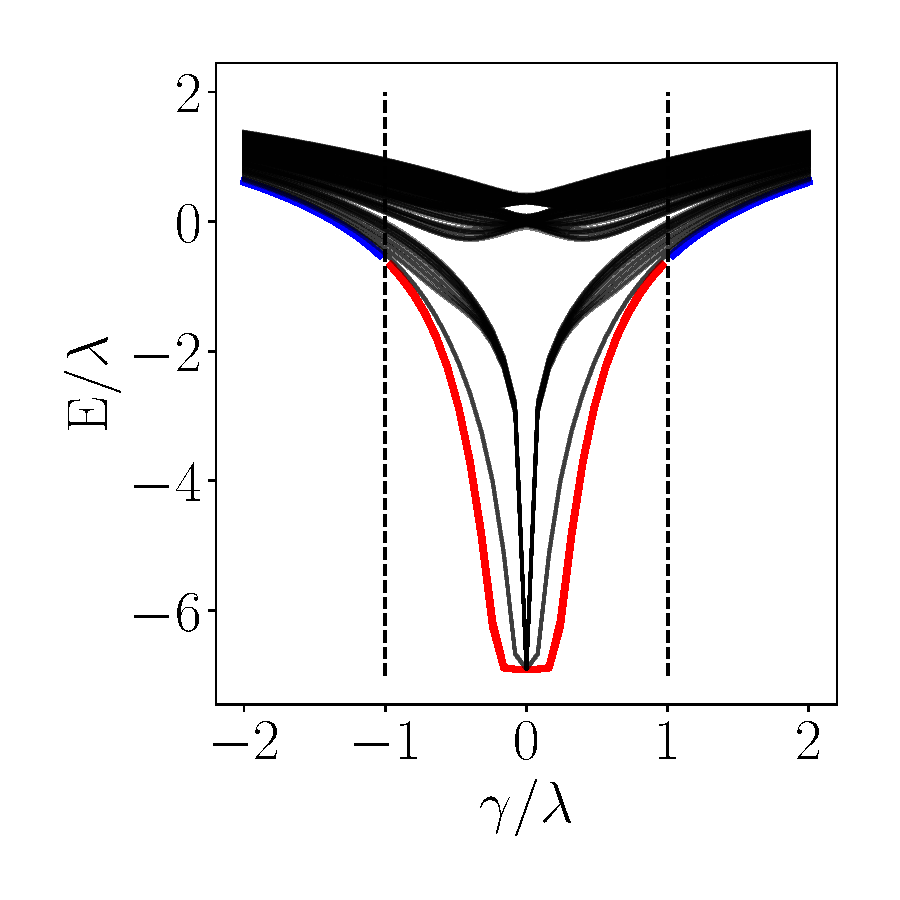
\includegraphics[width=\textwidth]{Imagenes/Resultados_Hoti_Fractal/bands_square_shh_log0.1.pdf}
             \label{}
         \end{subfigure}\hspace*{-0.5em}
         \begin{subfigure}[b!]{0.4 \textwidth}
             \caption{}
             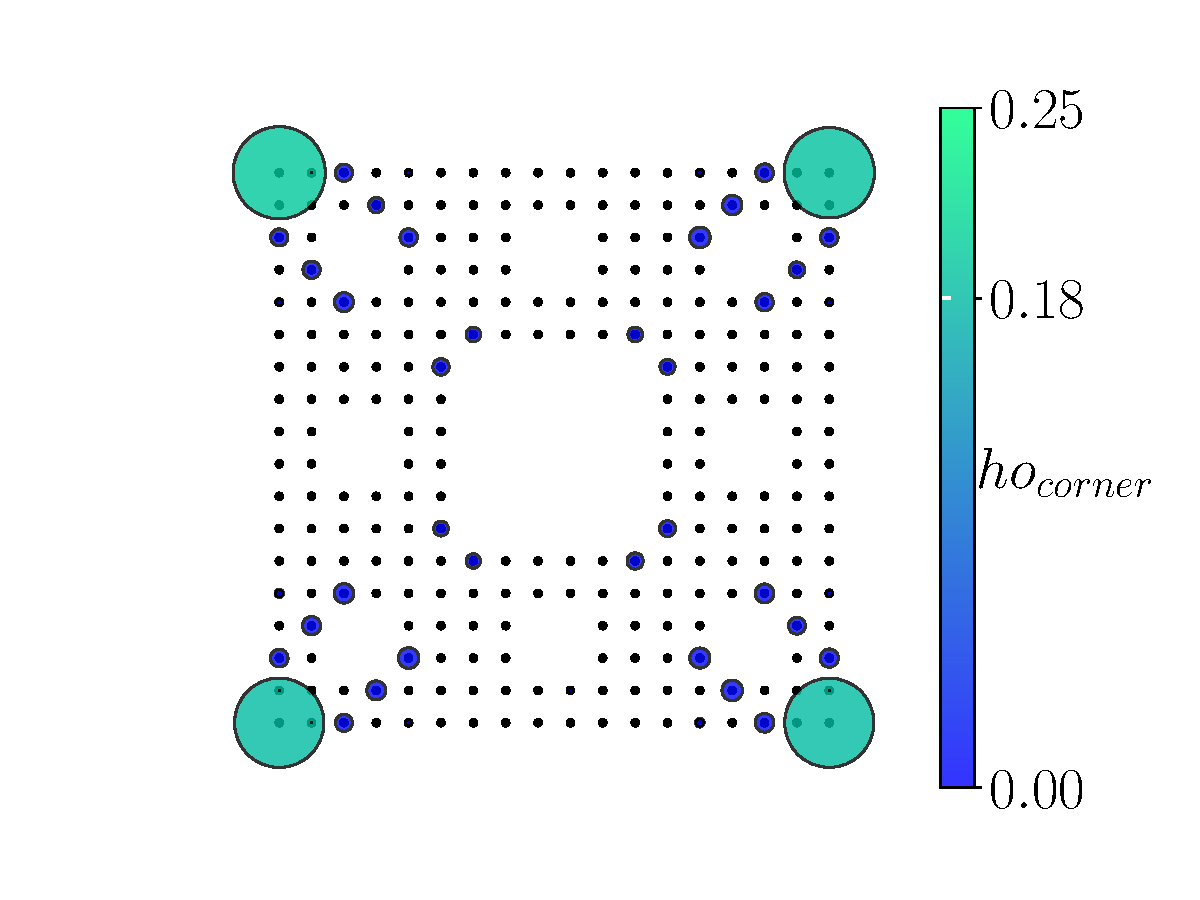
\includegraphics[width=\textwidth]{Imagenes/Resultados_Hoti_Fractal/proyection_square_0.1.pdf}
             \label{}
         \end{subfigure}\hspace*{-0.5em}
     \end{minipage}\vspace*{-2.5em}
     
     \begin{minipage}[h!]{0.9\textwidth}
         \begin{subfigure}[b!]{0.3 \textwidth}
             \caption{}
             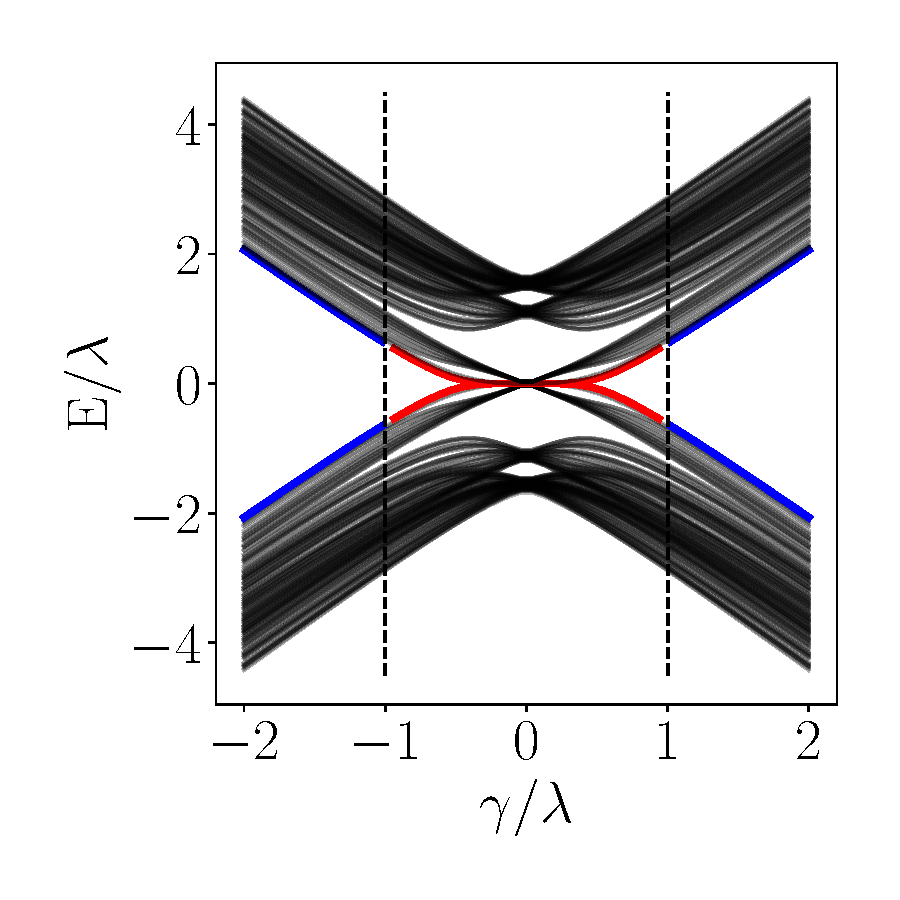
\includegraphics[width=\textwidth]{Imagenes/Resultados_Hoti_Fractal/bands_square_shh_0.2.pdf}
             \label{}
         \end{subfigure}\hspace*{-0.5em}
         \begin{subfigure}[b!]{0.3 \textwidth}
             \caption{}
             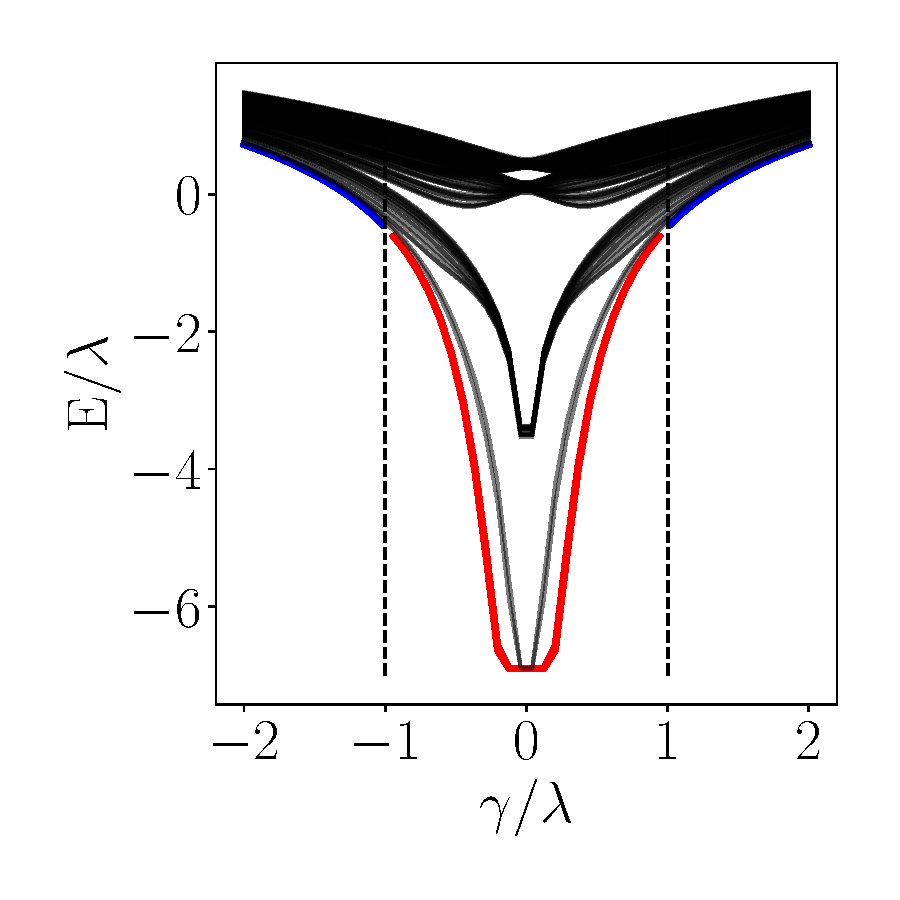
\includegraphics[width=\textwidth]{Imagenes/Resultados_Hoti_Fractal/bands_square_shh_log0.2.pdf}
             \label{}
         \end{subfigure}\hspace*{-0.5em}
         \begin{subfigure}[b!]{0.4 \textwidth}
             \caption{}
             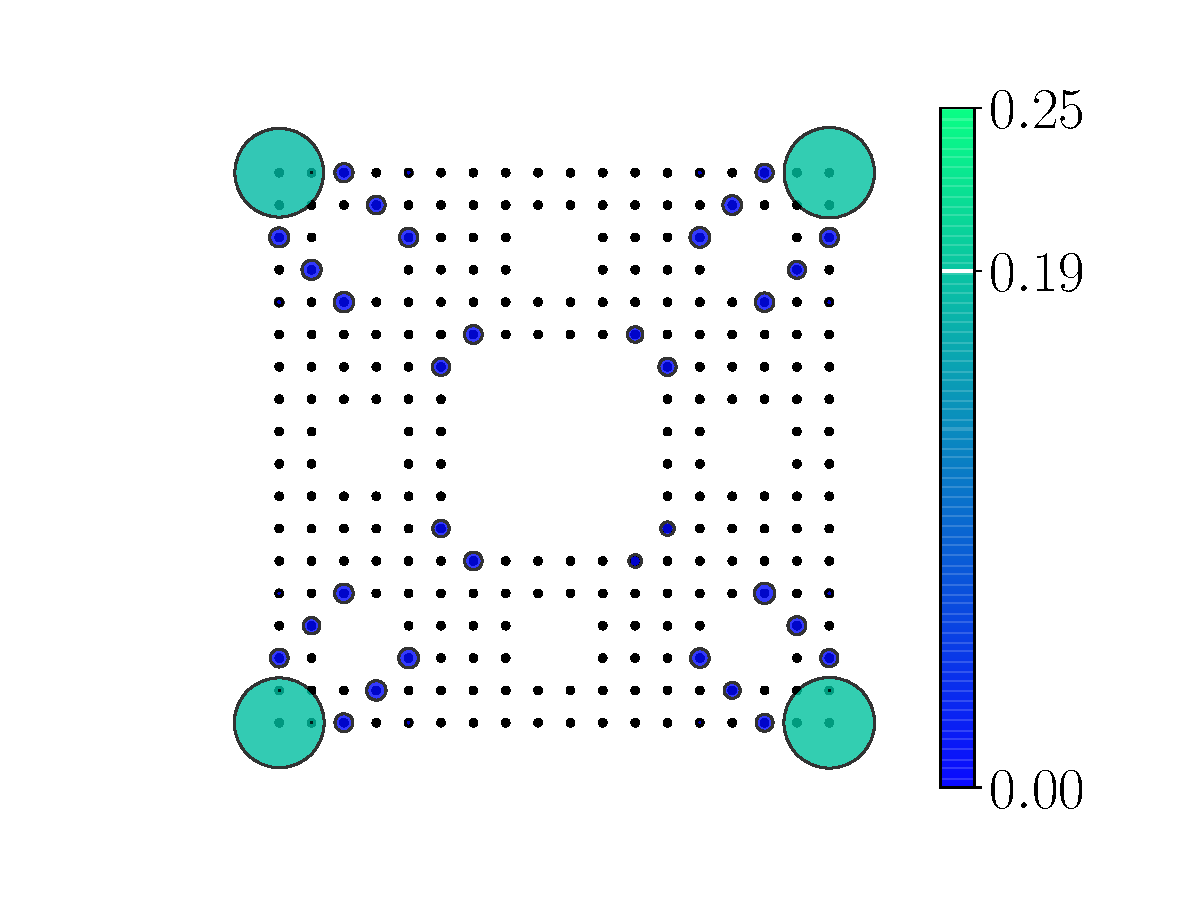
\includegraphics[width=\textwidth]{Imagenes/Resultados_Hoti_Fractal/proyection_square_0.2.pdf}
             \label{}
         \end{subfigure}\hspace*{-0.5em}
     \end{minipage}\vspace*{-2.5em}
     
     \begin{minipage}[h!]{0.9\textwidth}
         \begin{subfigure}[b!]{0.3 \textwidth}
             \caption{}
             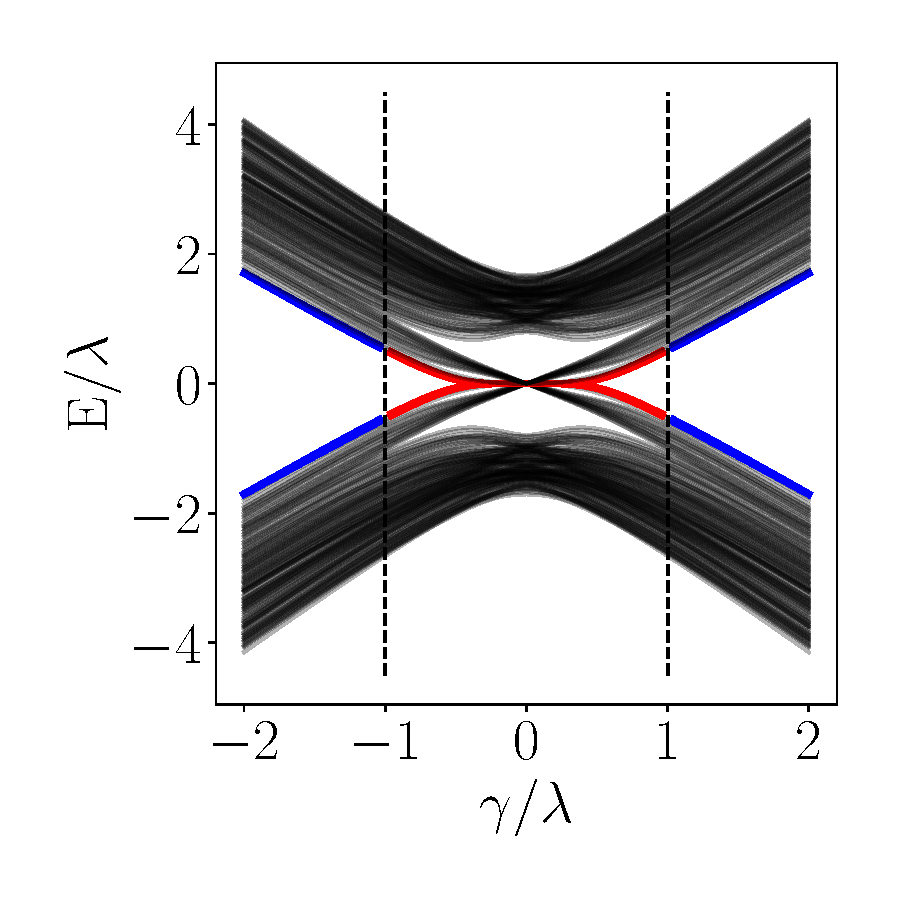
\includegraphics[width=\textwidth]{Imagenes/Resultados_Hoti_Fractal/bands_square_shh_0.3.pdf}
             \label{}
         \end{subfigure}\hspace*{-0.5em}
         \begin{subfigure}[b!]{0.3 \textwidth}
             \caption{}
             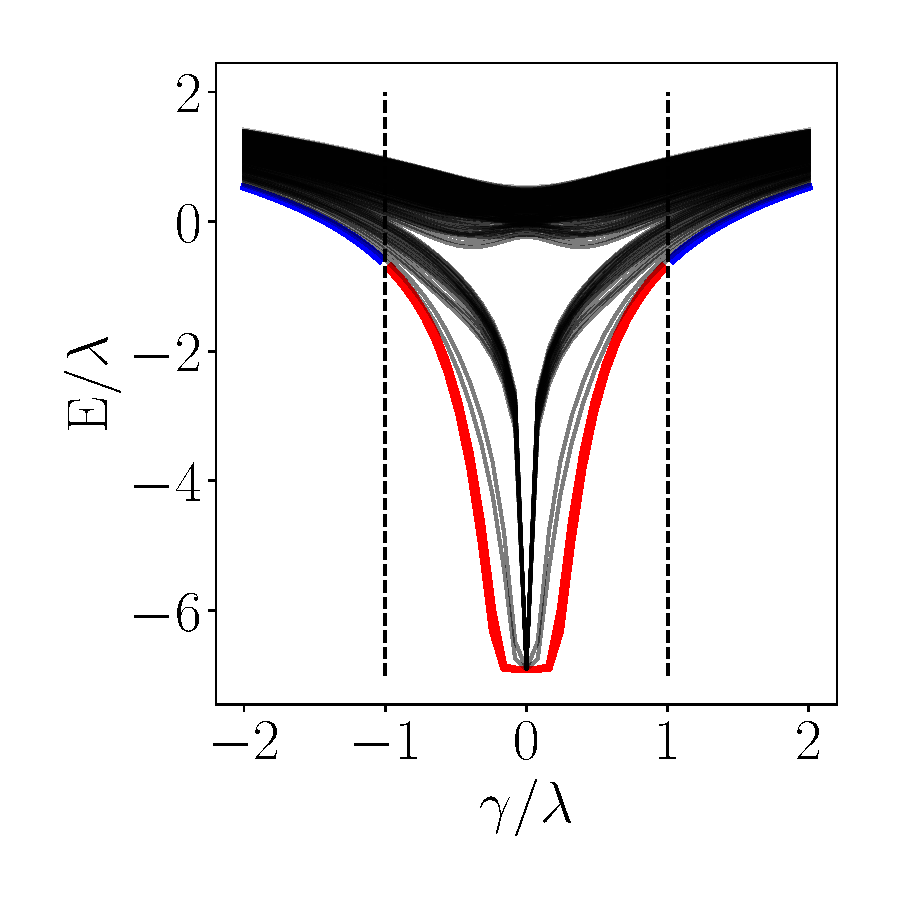
\includegraphics[width=\textwidth]{Imagenes/Resultados_Hoti_Fractal/bands_square_shh_log0.3.pdf}
             \label{}
         \end{subfigure}\hspace*{-0.5em}
         \begin{subfigure}[b!]{0.4 \textwidth}
             \caption{}
             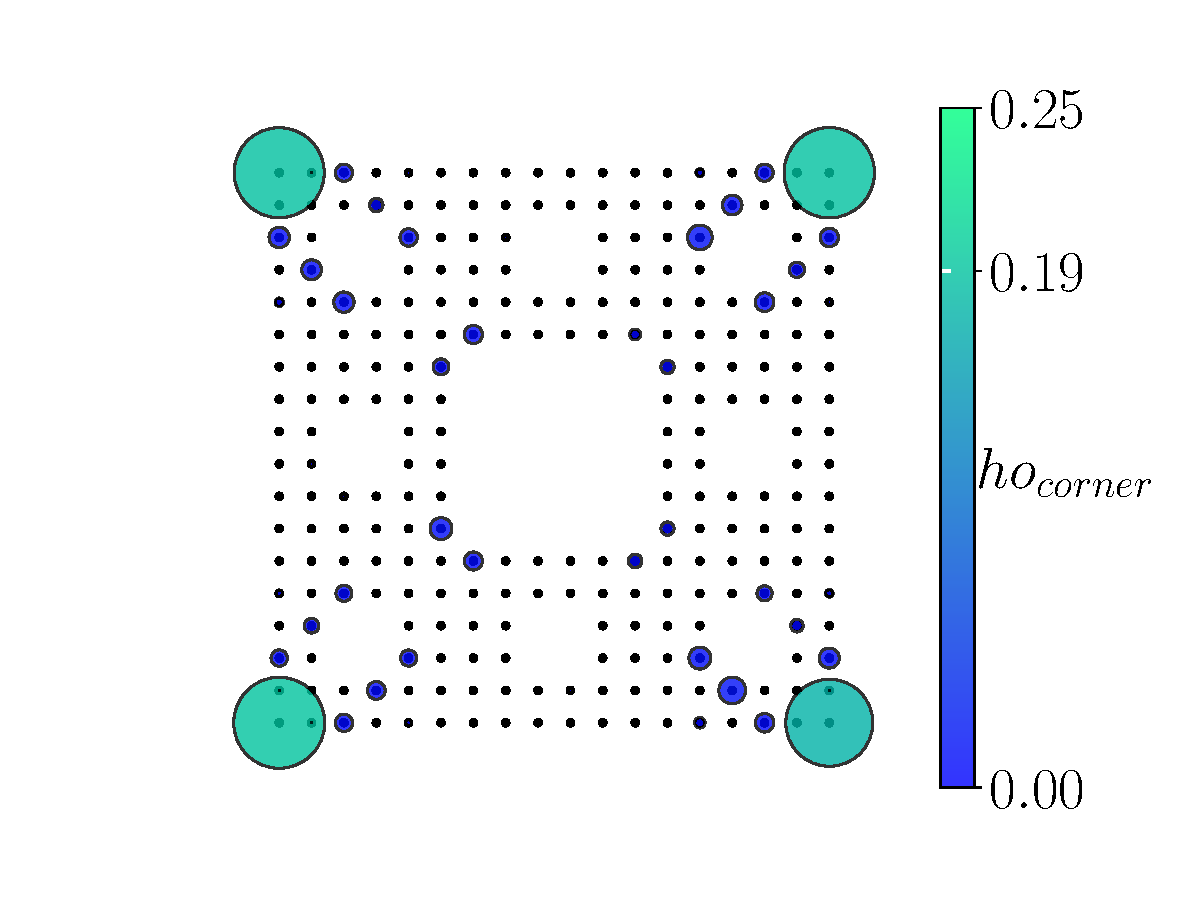
\includegraphics[width=\textwidth]{Imagenes/Resultados_Hoti_Fractal/proyection_square_0.3.pdf}
             \label{}
         \end{subfigure}\hspace*{-0.5em}
     \end{minipage}\vspace*{-2.5em}
     
      \begin{minipage}[h!]{0.9\textwidth}
         \begin{subfigure}[b!]{0.3 \textwidth}
             \caption{}
             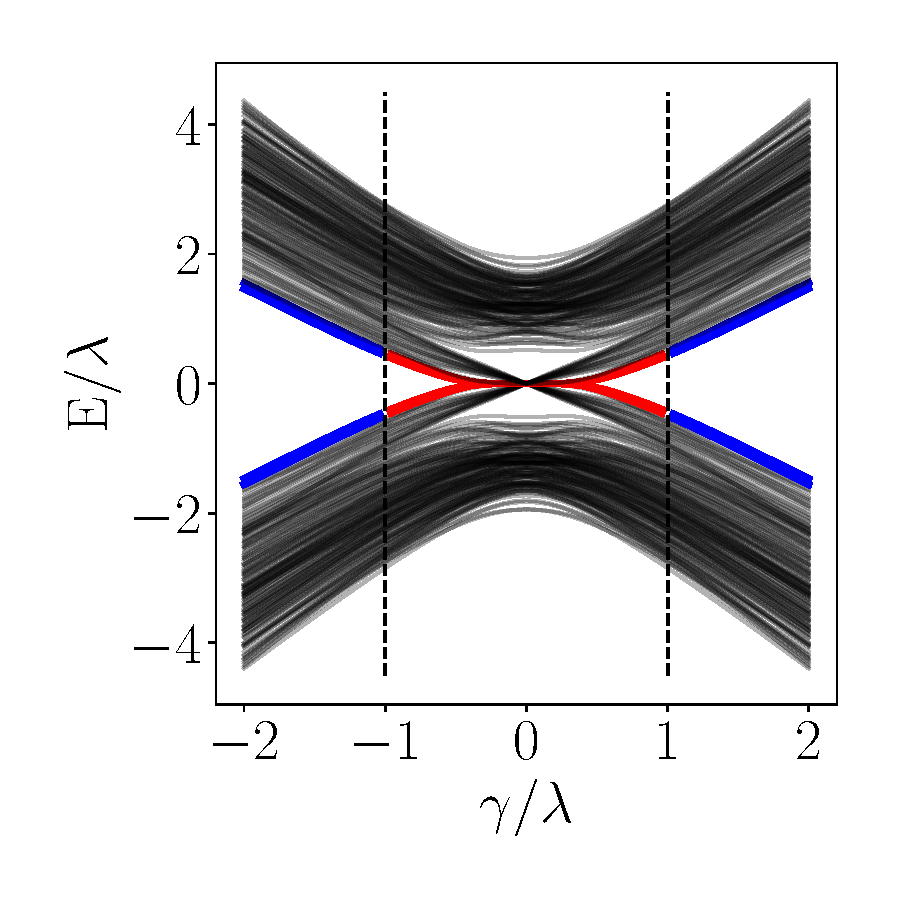
\includegraphics[width=\textwidth]{Imagenes/Resultados_Hoti_Fractal/bands_square_shh_0.5.pdf}
             \label{}
         \end{subfigure}\hspace*{-0.5em}
         \begin{subfigure}[b!]{0.3 \textwidth}
             \caption{}
             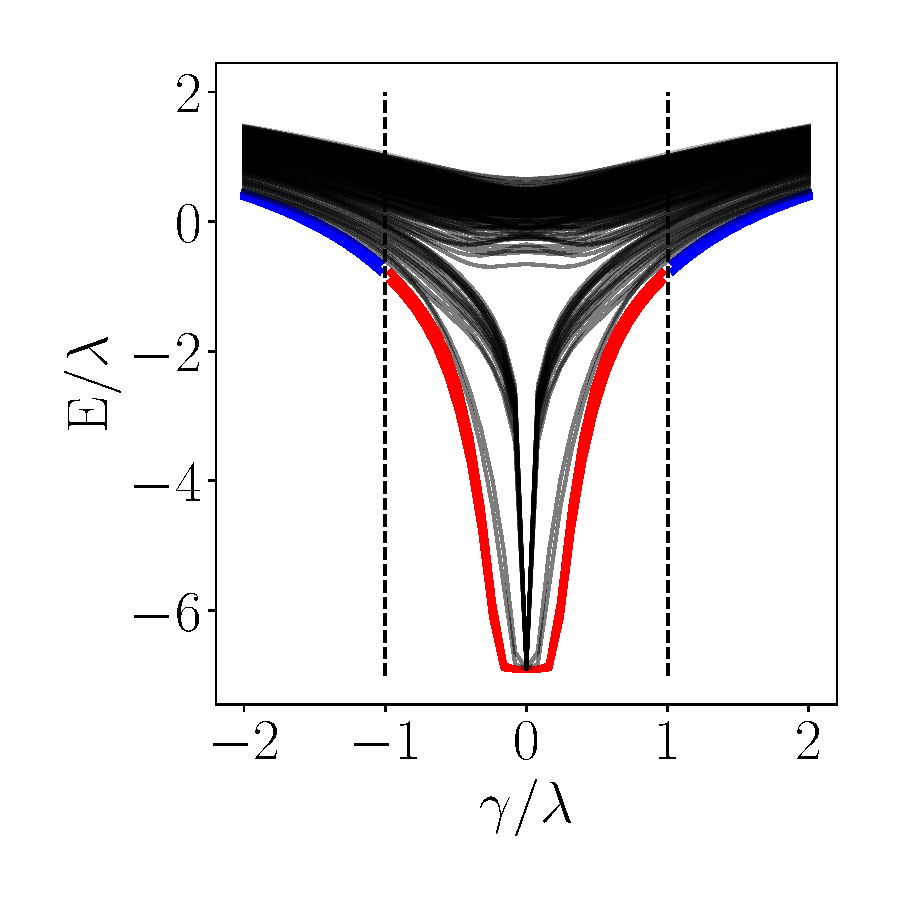
\includegraphics[width=\textwidth]{Imagenes/Resultados_Hoti_Fractal/bands_square_shh_log0.5.pdf}
             \label{}
         \end{subfigure}\hspace*{-0.5em}
         \begin{subfigure}[b!]{0.4 \textwidth}
             \caption{}
             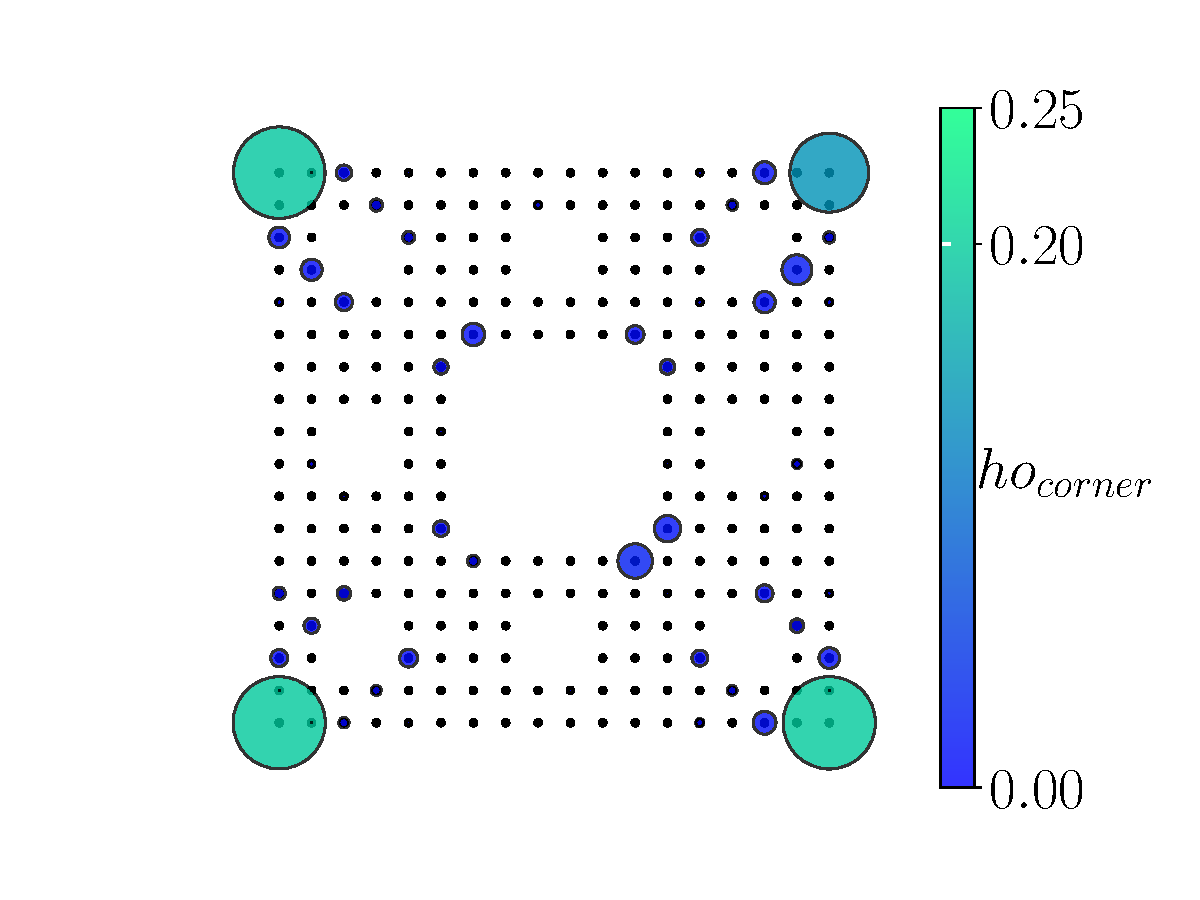
\includegraphics[width=\textwidth]{Imagenes/Resultados_Hoti_Fractal/proyection_square_0.5.pdf}
             \label{}
         \end{subfigure}\hspace*{-0.5em}
     \end{minipage}\vspace*{-2em}
     
     
    \caption{En la columna derecha se muestra el espectro de energías en una red cuadrada como función de $\gamma/\lambda $ con un desorden aleatorio en los parámetros de salto, de tamaño $\delta$. Las lineas rojas corresponden a los cuatro estados degenerados que representan los estados localizados en las esquinas. En la columna central se muestra el espectro de energías en escala logarítmica. En la columna izquierda se muestra la densidad de probabilidad de la fase no trivial donde $\gamma = 1 + \delta ,\, \, \lambda = 4.5 + \delta $.  }
    \label{fig:para_proy_Delta_fractal}
\end{figure}